\documentclass{article}

\usepackage[utf8]{inputenc}

\usepackage{scrextend}

\usepackage{geometry}
\geometry{
	a4paper,
	total={170mm,257mm},
	left=20mm,
	top=20mm,
}

\usepackage{graphicx}
\usepackage[portuguese]{babel}
\usepackage{subfig}


\usepackage{listings}
\usepackage{xcolor}

\definecolor{codegreen}{rgb}{0,0.6,0}
\definecolor{codegray}{rgb}{0.5,0.5,0.5}
\definecolor{codepurple}{rgb}{0.58,0,0.82}
\definecolor{backcolour}{rgb}{0.95,0.95,0.92}

\lstdefinestyle{mystyle}{
	backgroundcolor=\color{backcolour},   
	commentstyle=\color{codegreen},
	keywordstyle=\color{magenta},
	numberstyle=\tiny\color{codegray},
	stringstyle=\color{codepurple},
	basicstyle=\ttfamily\footnotesize,
	breakatwhitespace=false,         
	breaklines=true,                 
	captionpos=b,                    
	keepspaces=true,                 
	numbers=left,                    
	numbersep=5pt,                  
	showspaces=false,                
	showstringspaces=false,
	showtabs=false,                  
	tabsize=2
}

\lstset{style=mystyle}

%\usepackage{indentfirst}
\setlength{\parindent}{1.5cm}% too much in my eyes delete this
% line and use the default ...


\title{
	Escondendo uma mensagem em uma imagem (trabalho 1) \\
	\Large Introdução ao Processamento de Imagem Digital \\
	Randerson A. Lemos (103897)
	2022-1S
}

\date{\vspace{-5ex}}

\begin{document}
  \pagenumbering{gobble}
  \maketitle

%
%%
\section{Introdução}
A esteganografia é a área de conhecimento que se dedica a estudar técnicas de ocultação de informações (por exemplo, mensagens) em imagens sem que estas sofram alterações perceptíveis ao olho humano. A esteganografia, neste trabalho, será aplicada por meio da substituição dos bits menos significativos dos pixels das imagens escolhidas pelos bits das mensagens de interesse que se deseja ocultar. A seguir teremos três seções, a de Solução, a de Resultado e a de Conclusão. Na seção de Solução, detalhes técnicos, de usabilidade e de decisões da solução proposta são fornecidos. Na seção de Resultado, os principais resultados são apresentados. Na seção de Conclusão, há não apenas a apresentação de conclusões, mas também de discussões.

%
%%
\section{Solução}
A solução utiliza a linguagem de programação Python e conta com o auxílio do gerenciador de projetos e pacotes Conda. Assumindo que o usuário tenha o Conda instalado em sua máquina, a configuração do projeto pode ser feita pela execução do comando \lstinline{conda env create -f environment.yml} a partir da pasta do projeto \textbf{trab1}. Esse comando cria o ambiente de trabalho \textbf{mc920-trab1} e instala os seguintes módulos: opencv, numpy, scipy, pandas, matplotlib. Finalizada a configuração do ambiente de trabalho em questão, o usuário deve executar o comando \lstinline{source source.sh}\footnote{O comando que configura o ambiente de trabalho mc920-trab1 precisa ser executado apenas um vez. Assim sendo, depois que este ambiente está configurado, o usuário precisa apenas executar o comando \lstinline{source source.sh}} para carregar as variáveis de ambiente adequadas e, assim, poder usar os programas do projeto dentro do próprio ambiente de trabalho recém configurado. 

Dos arquivos presentes na pasta do projeto \textbf{trab1}, destacam-se as pastas \textbf{png}, \textbf{tex}, \textbf{txt} e os programas \textbf{codificar.py}, \textbf{decodificar.py}, \textbf{mostrar\_planos.py}. A pasta \textbf{png} contém imagens no formato png que podem ser utilizadas como esconderijos das mensagens a serem ocultadas. A pasta \textbf{txt} contém exemplos de textos que podem ser utilizados no processo de ocultação de suas mensagens. A pasta \textbf{tex} contém os arquivos Latex deste relatório. As informações pertinentes dos programas \textbf{codificar.py}, \textbf{decodificar.py}, \textbf{mostrar\_planos.py} são detalhadas a seguir.

%
\subsection{Codificar.py}
O programa \textbf{codificar.py} é responsável por ocultar uma mensagem de interesse em uma imagem escolhida que deve ser colorida e estar no formato png. Para ser executado, esse programa precisa receber os parâmetros \textbf{imagem\_entrada}, \textbf{texto\_entrada}, e \textbf{planos\_bits}:

\begin{itemize}
	\item ao parâmetro \textbf{imagem\_entrada} deve-se fornecer o nome do arquivo da imagem a ser utilizada como `bau' da mensagem que se deseja esconder;
	\item ao parâmetro \textbf{texto\_entrada} deve-se fornecer o nome do arquivo do texto que contém a mensagem que
	se deseja esconder;
	\item ao parâmetro \textbf{planos\_bits} deve-se fornecer os planos de bits menos significativos dos pixels da imagem escolhida que serão utilizados para guardar os bits da mensagem de interesse. Os valores esperados para esse parâmetro são: 0, ou 1, ou 2, ou combinações desses valores separados por ‘:’. Quando mais de um plano de bits são passados ao programa pelo parâmetro \textbf{planos\_bits}, ocorre a ordenação em ordem crescente desses planos de modo que a utilização dos bits dos pixels da imagem se dê sempre do plano de bits menos significativo para o mais significativo.
\end{itemize}

\noindent
O texto de entrada que contem a mensagem a ser escondida na imagem escolhida deve apresentar um código de \textit{end of file} para que o processo subsequente de decodificação consiga identificar o final de mensagem. Aqui, o código escolhido é \textbf{!@\#FIM\#@!}. A combinação dos caracteres desse código foi pensada de modo que uma possível aparição não intencional de tal código ao longo do texto seja significativamente improvável.

Exemplos de como utilizar o programa \textbf{codificar.py} utilizando os recursos contidos dentro do próprio projeto são:

\lstinline{python3 codificar.py -imagem_entrada=png/watch.png -texto_entrada=txt/texto1.txt -planos_bits=2};

\lstinline{python3 codificar.py -imagem_entrada=png/watch.png -texto_entrada=txt/texto1.txt -planos_bits=1:2};

\lstinline{python3 codificar.py -imagem_entrada=png/watch.png -texto_entrada=txt/texto1.txt -planos_bits=0:1:2}.

\noindent
Após executado, o programa \textbf{codificar.py} gera uma imagem de saída. Esse imagem nada mais é que a imagem de entrada contendo a mensagem do texto de entrada oculta nos seus bits menos significativos de acordo com os planos de bits passados pelo usuário. Essa imagem de saída é salva automaticamente na pasta \textbf{out} que está dentro da pasta do projeto \textbf{trab1}. Se a imagem de entrada tem o nome \textbf{img\_ent.png} a imagem de saída apresentará o nome \textbf{img\_ent\underline{m\_planoX}.png}, onde o letra X é um \textit{placeholder} para os números dos planos de bits escolhidos pelo usuário.

Para demais informações acerca das implementações ou algoritmos utilizados, consultar o código fonte. Lá existem comentários que abrangem esse tipo de informação.

%
\subsection{Decodificar.py}
O programa \textbf{decodificar.py} é responsável por recuperar a mensagem escondida em um imagem previamente codificada com esse mensagem pelo programa \textbf{codificar.py}. Para ser executado, esse programa precisa receber os parâmetros \textbf{imagem\_entrada} e \textbf{planos\_bits}:

\begin{itemize}
	\item ao parâmetro \textbf{imagem\_entrada} deve-se fornecer o nome do arquivo da imagem que possui uma mensagem escondida cujo conteúdo se deseja recuperar;
	\item ao parâmetro \textbf{planos\_bits} deve-se fornecer os valores numéricos dos planos de bits nos quais os bits da mensagem escondida foram guardados. Essa parâmetro aceita os seguintes valores: 0, ou 1, ou 2, ou combinações desses valores separados por `:'.
\end{itemize}

\noindent
Exemplos de como executar o programa \textbf{decodificar.py} utilizando os recursos\footnote{É necessário que o comando adequado do programa codificar.py tenha sido executado.\label{refnote}} contidos dentro do próprio projeto são:

\lstinline{python3 decodificar.py -imagem_entrada=out/watchm_plano2.png -planos_bits=2};

\lstinline{python3 decodificar.py -imagem_entrada=out/watchm_plano01.png -planos_bits=0:1};

\lstinline{python3 decodificar.py -imagem_entrada=out/watchm_plano012.png -planos_bits=0:1:2}.

\noindent
Após executado, o programa \textbf{decodificar.py} é responsável por gerar um arquivo de texto contendo a mensagem que estava escondida na imagem repositório. Esse texto é salvo automaticamente na pasta \textbf{out} que está dentro da pasta do projeto \textbf{trab1}. Se a imagem com a mensagem escondida tiver o nome \textbf{img\_entm\_planoX.png} o arquivo texto da mensagem terá o nome \textbf{img\_entm\_planoX.txt}.

Para demais informações acerca das implementações ou algoritmos utilizados, consultar o código fonte. Lá existem comentários que abrangem esse tipo de informação.

%
\subsection{Mostrar\_planos.py}
O programa \textbf{mostrar\_planos.py} é responsável por gerar mapas de bits dos três canais (RGB) de uma imagem selecionada. Para funcionar esse programa precisa receber os parâmetros \textbf{imagem\_entrada} e \textbf{planos\_bits}:

\begin{itemize}
	\item ao parâmetro \textbf{imagem\_entrada} deve-se fornecer o nome do arquivo da imagem que se deseja visualizar os planos de bits;
	\item ao parâmetro \textbf{planos\_bits} deve-se fornecer os valores numéricos dos planos de bits que se deseja visualizar. Essa parâmetro aceita valores de 0 (referente ao plano de bits menos significativo) até 7 (referente ao plano de bits mais significativo). Para gerar imagens de múltiplos planos de bits, basta passar os valores dos planos de interesse separados por `:'.
\end{itemize}

\noindent
Exemplos de como executar o programa \textbf{mostrar\_planos.py} utilizando os recursos\footref{refnote} contidos dentro do próprio projeto são:

\lstinline{python3 mostrar_planos.py -imagem_entrada=out/watchm_plano12.png -planos_bits=3},

\lstinline{python3 mostrar_planos.py -imagem_entrada=out/watchm_plano12.png -planos_bits=0:1:2:7}.

\noindent
Após executado, o programa \textbf{mostrar\_planos.py} gera imagens dos planos de bits passados pelo usuário dos canais RGB da imagem selecionada. Essa imagem de saída é salva automaticamente na pasta \textbf{out} que está dentro da pasta do projeto \textbf{trab1}. Se a imagem de entrada tem o nome \textbf{img\_entm\_planoX.png}, as imagens de saída apresentarão nome segundo o padrão \textbf{img\_entm\_planoX\underline{\_plano\_bits\_Y\_Z}.png} em que Y é o \textit{placeholder} para o número do plano de bits apresentado na imagem e Z é o \textit{placeholder} para os canais (R, G ou B) dos planos de bits.

Para demais informações acerca das implementações ou algoritmos utilizados, consultar o código fonte. Lá existem comentários que abrangem esse tipo de informação.

%
%%
\section{Resultado}
Os resultados levantados são provenientes da aplicação dos programas \textbf{codificar.py}, \textbf{decodificar.py}, \textbf{mostar\_planos.py} sobre a imagens apresentadas na Figura \ref{fig:imagem:entrada}. 

\begin{figure}[htp]%
	\centering
	\subfloat[\centering Baboon (png/baboon.png)]{{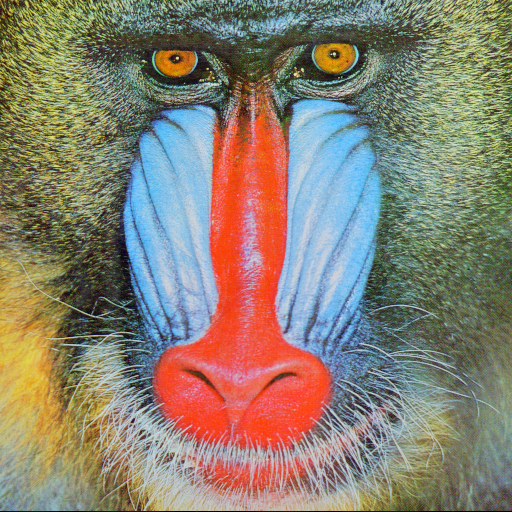
\includegraphics[width=5cm]{../png/baboon.png} }}%
	\qquad
	\subfloat[\centering Watch (png/watch.png)]{{
\includegraphics[width=5cm]{../png/watch.png} }}%
	\caption{Imagens utilizadas para aplicação da solução de esteganografia.}%
	\label{fig:imagem:entrada}%
\end{figure}

\noindent
Ambas as imagens estão no formato requerido (png) e estão localizadas na pasta \textbf{png} que está dentro da pasta do projeto \textbf{trab1}. A imagem Baboon apresenta dimensões de 512x512. A imagem Watch apresenta dimensões de 1024x768. 

Duas mensagem serão aplicadas em cada uma desses imagens (em momentos diferentes). Uma mensagem é \textbf{TAMO JUNTO!!!} que está armazenada no arquivo \textbf{texto1.txt}, localizado na pasta \textbf{txt} que está dentro da pasta do projeto \textbf{trab1}. Importante salientar que nessa mensagem também há o conjunto de caracteres \textbf{!@\#FIM\#@!} que codificam o final de mensagem. A outra mensagem é uma sequencia de letras `a's cujo tamanho é suficiente para encher um plano de bits dos três canais completamente da imagem Baboon. Essa mensagem está armazenada no arquivo \textbf{texto\_longo\_1.txt} que está também localizada na pasta \textbf{txt}.

Os comandos utilizados para ocultação da mensagem contida no arquivo \textbf{texto1.txt} foram:

\lstinline{python3 codificar.py -imagem_entrada=png/baboon.png -texto_entrada=txt/texto1.txt -planos_bits=0};

\lstinline{python3 codificar.py -imagem_entrada=png/watch.png -texto_entrada=txt/texto1.txt -planos_bits=0}.

\noindent
As imagens resultantes com a mensagem escondida estão apresentadas na Figura \ref{fig:imagem:saida}.
	
\begin{figure}[htp]%
\centering
\subfloat[\centering Baboon com mensagem escondida (out/baboonm\_plano0\_texto1.png)]{{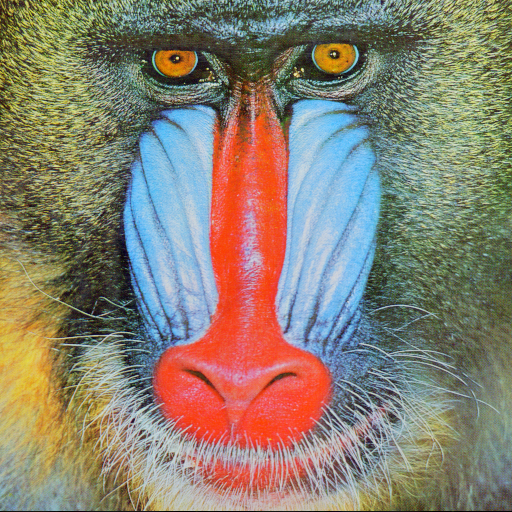
\includegraphics[width=5cm]{../out/baboonm_plano0_texto1.png} }}%
\qquad
\subfloat[\centering Watch com mensagem escondida (out/watchm\_plano0\_texto1.png)]{{
\includegraphics[width=5cm]{../out/watchm_plano0_texto1.png} }}%
\caption{Imagens que apresentam mensagem escondida do arquivo \textbf{texto1.txt}.}%
\label{fig:imagem:saida}%
\end{figure}	

\newpage\noindent
Os comandos utilizados para ocultação de mensagem contida no arquivo \textbf{texto\_longo\_1.txt} foram:

\lstinline{python3 codificar.py -imagem_entrada=png/baboon.png -texto_entrada=txt/texto_longo_1.txt -planos_bits=0};

\lstinline{python3 codificar.py -imagem_entrada=png/watch.png -texto_entrada=txt/texto_longo_1.txt -planos_bits=0}.

\noindent
As imagens resultantes com a mensagem escondida estão apresentadas na Figura \ref{fig:imagem:saida2}.

\begin{figure}[htp]%
	\centering
	\subfloat[\centering Baboon com mensagem escondida (/out/baboonm\_plano0\_texto\_longo\_1.png)]{{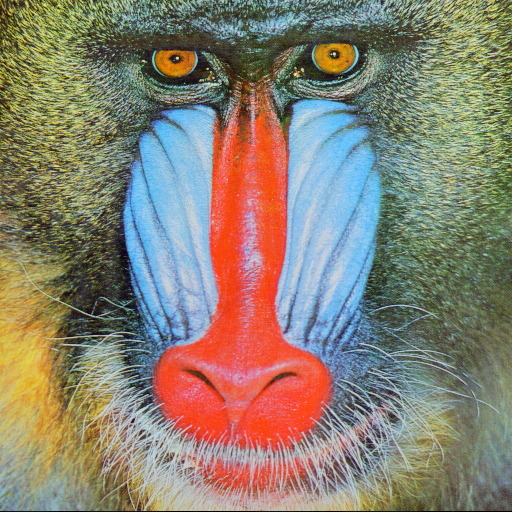
\includegraphics[width=5cm]{../out/baboonm_plano0_texto_longo_1.png} }}%
	\qquad
	\subfloat[\centering Watch com mensagem escondida (out/watchm\_plano0\_texto\_longo\_1.png)]{{
\includegraphics[width=5cm]{../out/watchm_plano0_texto_longo_1.png} }}%
	\caption{Imagens que apresentam mensagem escondida do arquivo do \textbf{texto\_longo\_1.txt}.}%
	\label{fig:imagem:saida2}%
\end{figure}


Nota-se que visualmente, essas imagens, apesar de modificadas pelos bits da mensagem escondida, não apresentam alterações visuais perceptíveis ao olho humano. Vamos visualizar os planos 0, 1, 2 e 7 dessas imagens para cada umas das duas mensagens \textbf{texto1.txt} e \textbf{texto\_longo\_1.txt}. 


\subsection{Planos de bits da imagem Baboon e Watch modifica pela mensagem contida no arquivo texto1.txt}

Começaremos visualizando os planos de bits da imagem do Baboon modificada. Os planos apresentados serão os 0, 1, 2, e 7 (0 menos significativo, 7 o mais significativo). As imagens dos planos de bits podem ser visualizadas na Figura \ref{fig:imagem:plano:baboon}.

\begin{figure}[htp]%
	\centering
	\subfloat[\centering Plano de bits 0 do canal R da Baboon com mensagem escondida]{{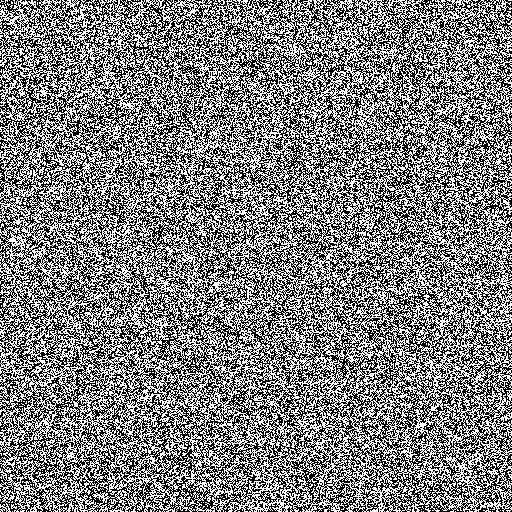
\includegraphics[width=3cm]{../out/baboonm_plano0_texto1_plano_bits_0_R.png} }}%
	\qquad
	\subfloat[\centering Plano de bits 0 do canal G da Baboon com mensagem escondida]{{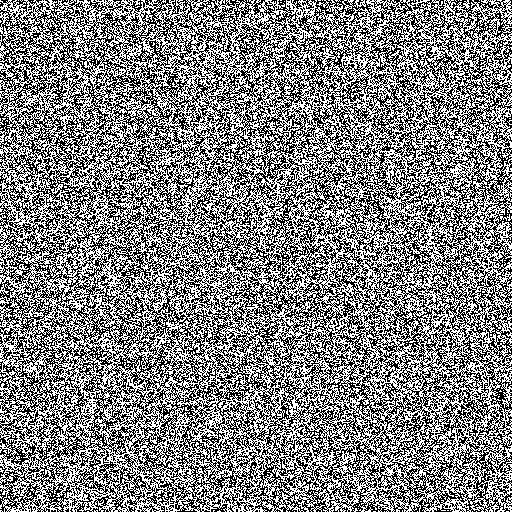
\includegraphics[width=3cm]{../out/baboonm_plano0_texto1_plano_bits_0_G.png} }}%
	\qquad
	\subfloat[\centering Plano de bits 0 do canal B da Baboon com mensagem escondida]{{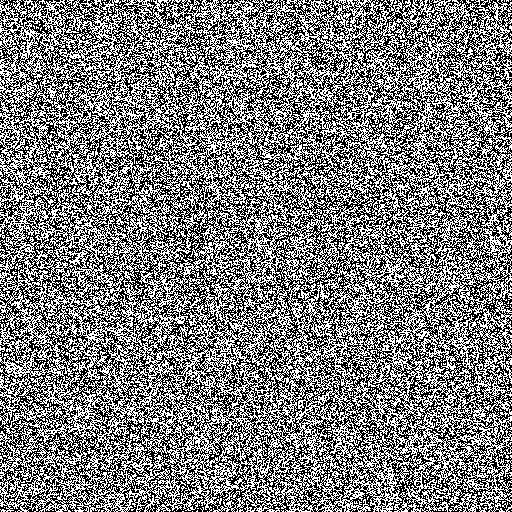
\includegraphics[width=3cm]{../out/baboonm_plano0_texto1_plano_bits_0_B.png} }}%
	
	\subfloat[\centering Plano de bits 1 do canal R da Baboon com mensagem escondida]{{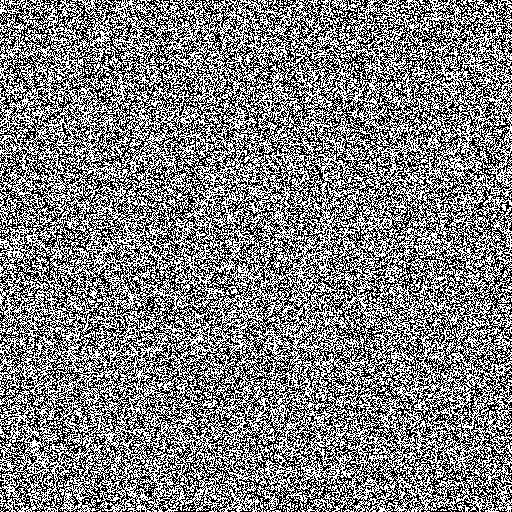
\includegraphics[width=3cm]{../out/baboonm_plano0_texto1_plano_bits_1_R.png} }}%
	\qquad
	\subfloat[\centering Plano de bits 1 do canal G da Baboon com mensagem escondida]{{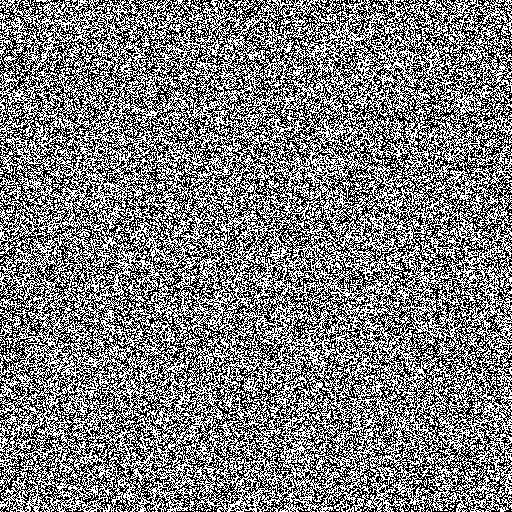
\includegraphics[width=3cm]{../out/baboonm_plano0_texto1_plano_bits_1_G.png} }}%
	\qquad
	\subfloat[\centering Plano de bits 1 do canal B da Baboon com mensagem escondida]{{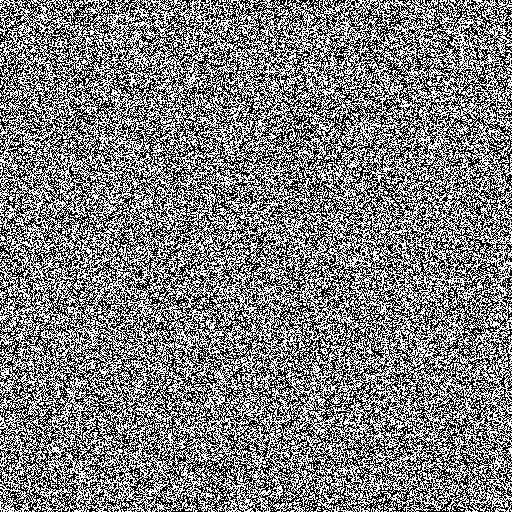
\includegraphics[width=3cm]{../out/baboonm_plano0_texto1_plano_bits_1_B.png} }}%
	
	\subfloat[\centering Plano de bits 2 do canal R da Baboon com mensagem escondida]{{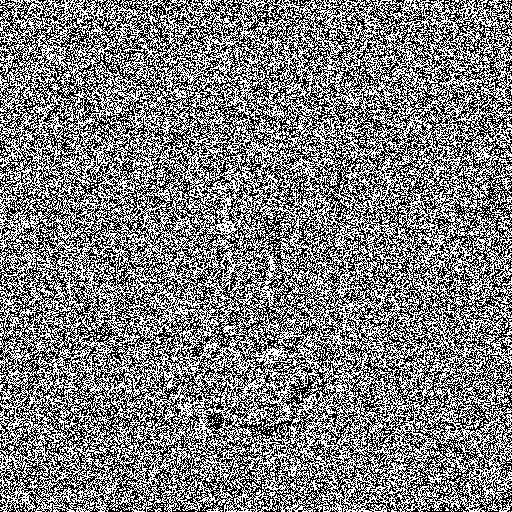
\includegraphics[width=3cm]{../out/baboonm_plano0_texto1_plano_bits_2_R.png} }}%
	\qquad
	\subfloat[\centering Plano de bits 2 do canal G da Baboon com mensagem escondida]{{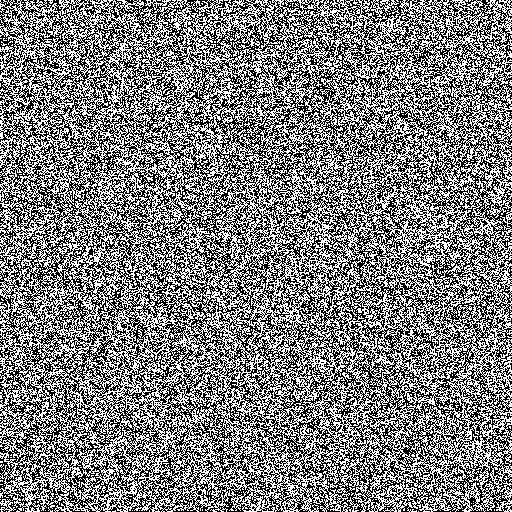
\includegraphics[width=3cm]{../out/baboonm_plano0_texto1_plano_bits_2_G.png} }}%
	\qquad
	\subfloat[\centering Plano de bits 2 do canal B da Baboon com mensagem escondida]{{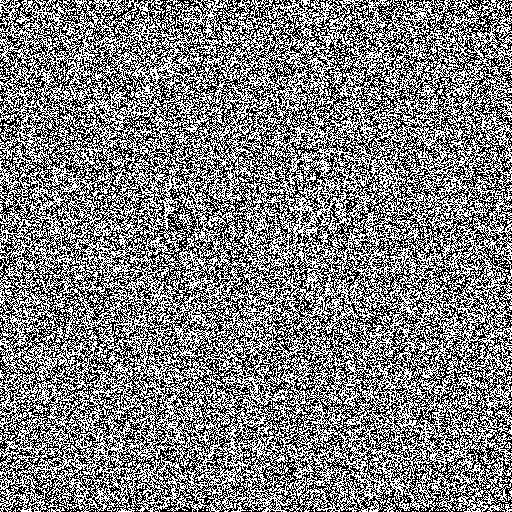
\includegraphics[width=3cm]{../out/baboonm_plano0_texto1_plano_bits_2_B.png} }}%
	
	\subfloat[\centering Plano de bits 7 do canal R da Baboon com mensagem escondida]{{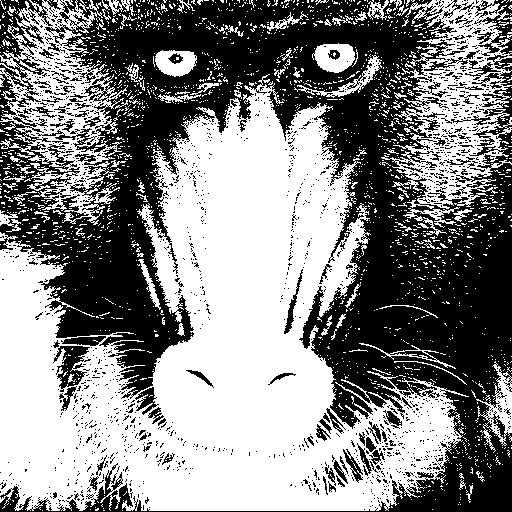
\includegraphics[width=3cm]{../out/baboonm_plano0_texto1_plano_bits_7_R.png} }}%
	\qquad
	\subfloat[\centering Plano de bits 7 do canal G da Baboon com mensagem escondida]{{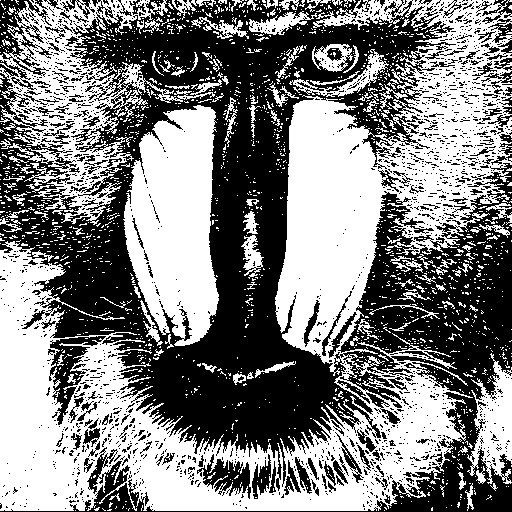
\includegraphics[width=3cm]{../out/baboonm_plano0_texto1_plano_bits_7_G.png} }}%
	\qquad
	\subfloat[\centering Plano de bits 7 do canal B da Baboon com mensagem escondida]{{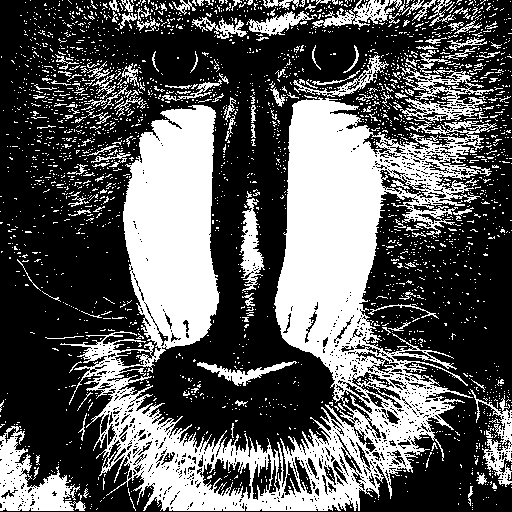
\includegraphics[width=3cm]{../out/baboonm_plano0_texto1_plano_bits_7_B.png} }}%

	\caption{Planos de bits da imagem do Baboon modificada pelos bits da mensagem do arquivo \textbf{texto1.txt}.}%
	\label{fig:imagem:plano:baboon}%
\end{figure}	


Para as imagens apresentadas na Figura \ref{fig:imagem:plano:baboon}, notamos que não é possível visualmente verificar que a imagem foi modificada a partir da análise visual dos seus planos de bits. Essa condição deve ser propiciada tanto pela ruído apresentado nos planos de bits menos significativos quanto pelo tamanho da mensagem que é pequeno. Também podemos perceber que os planos bits menos significativos carregam menos informações da composição da imagem do que os planos de bits mais significativos. Logo, é por isso que modificar esse bits (os menos significativos) não altera perceptivelmente a imagem de saída.

\newpage
Agora vamos verificar o planos de bits 0, 1, 2 e 7 da imagem Watch modificada. Esses planos de bits estão apresentados na Figura \ref{fig:imagem:plano:watch}. 

\begin{figure}[htp]%
	\centering
	\subfloat[\centering Plano de bits 0 do canal R da Watch com mensagem escondida]{{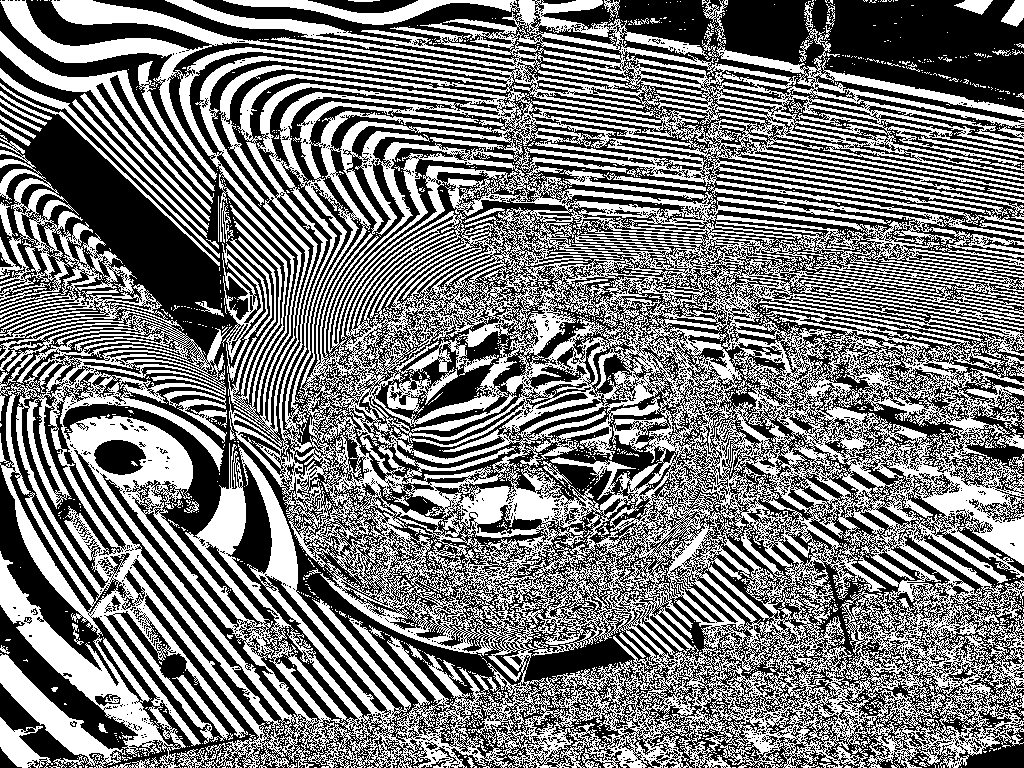
\includegraphics[width=3cm]{../out/watchm_plano0_texto1_plano_bits_0_R.png} }}%
	\qquad
	\subfloat[\centering Plano de bits 0 do canal G da Watch com mensagem escondida]{{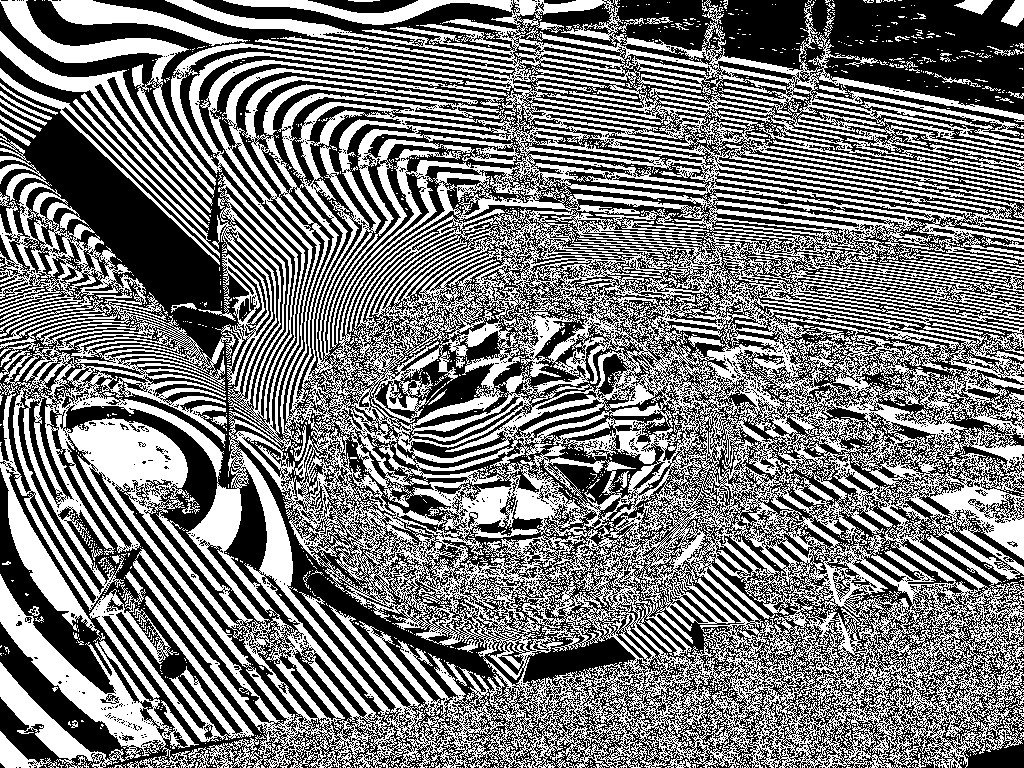
\includegraphics[width=3cm]{../out/watchm_plano0_texto1_plano_bits_0_G.png} }}%
	\qquad
	\subfloat[\centering Plano de bits 0 do canal B da Watch com mensagem escondida]{{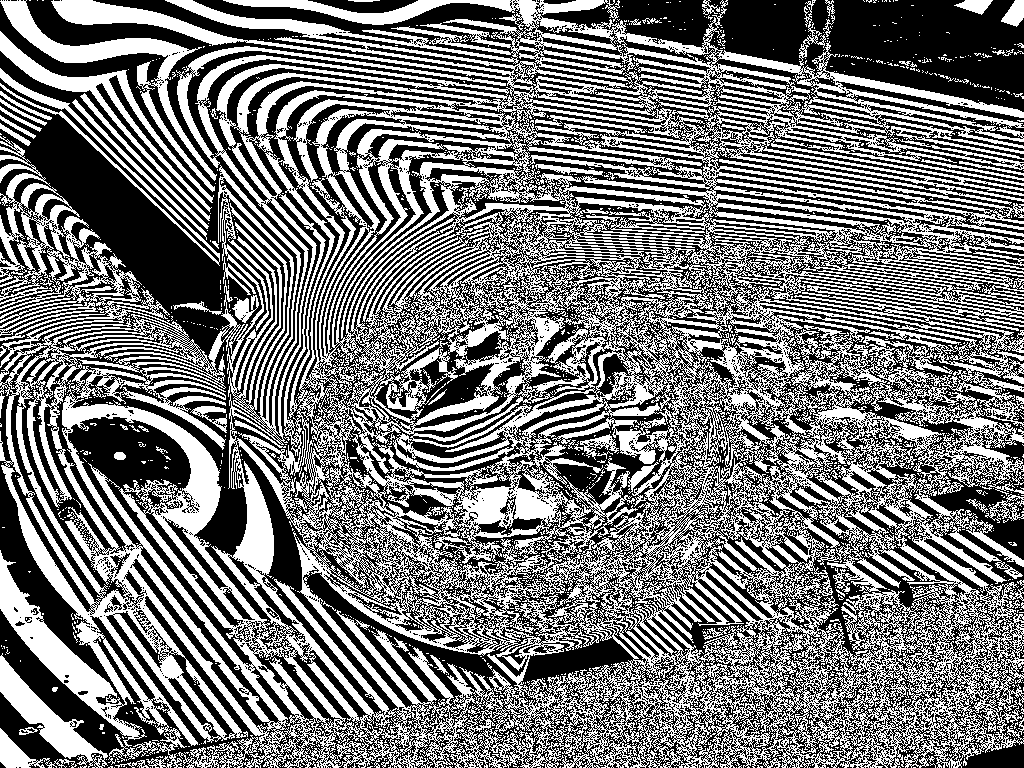
\includegraphics[width=3cm]{../out/watchm_plano0_texto1_plano_bits_0_B.png} }}%
	
	\subfloat[\centering Plano de bits 1 do canal R da Watch com mensagem escondida]{{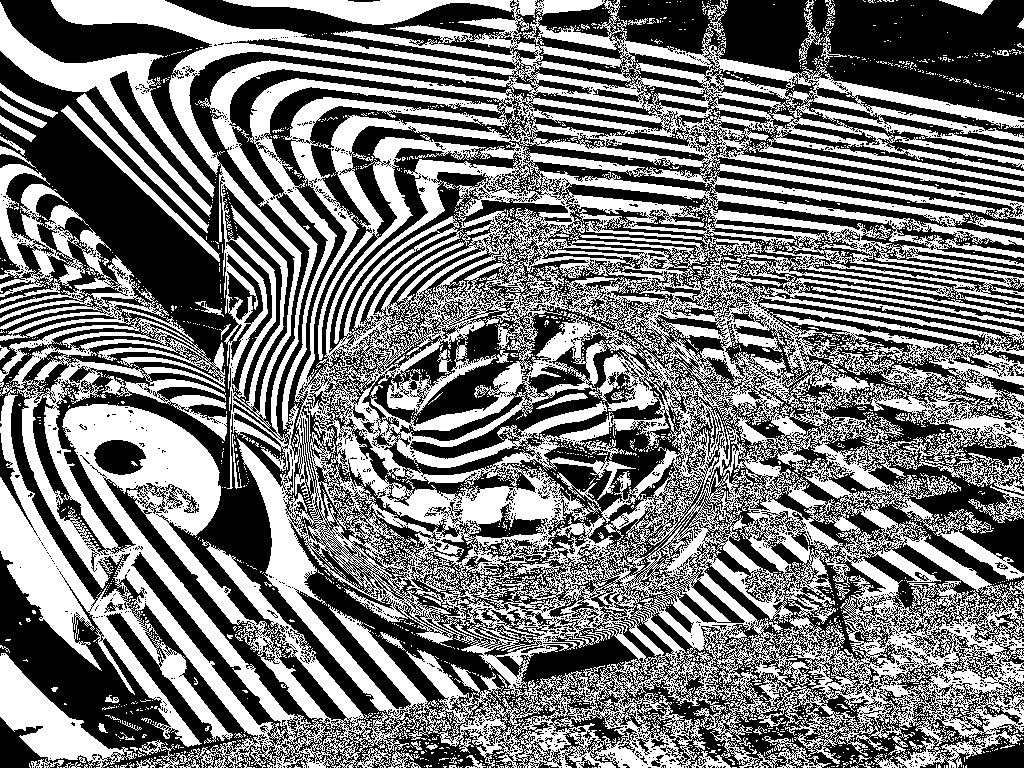
\includegraphics[width=3cm]{../out/watchm_plano0_texto1_plano_bits_1_R.png} }}%
	\qquad
	\subfloat[\centering Plano de bits 1 do canal G da Watch com mensagem escondida]{{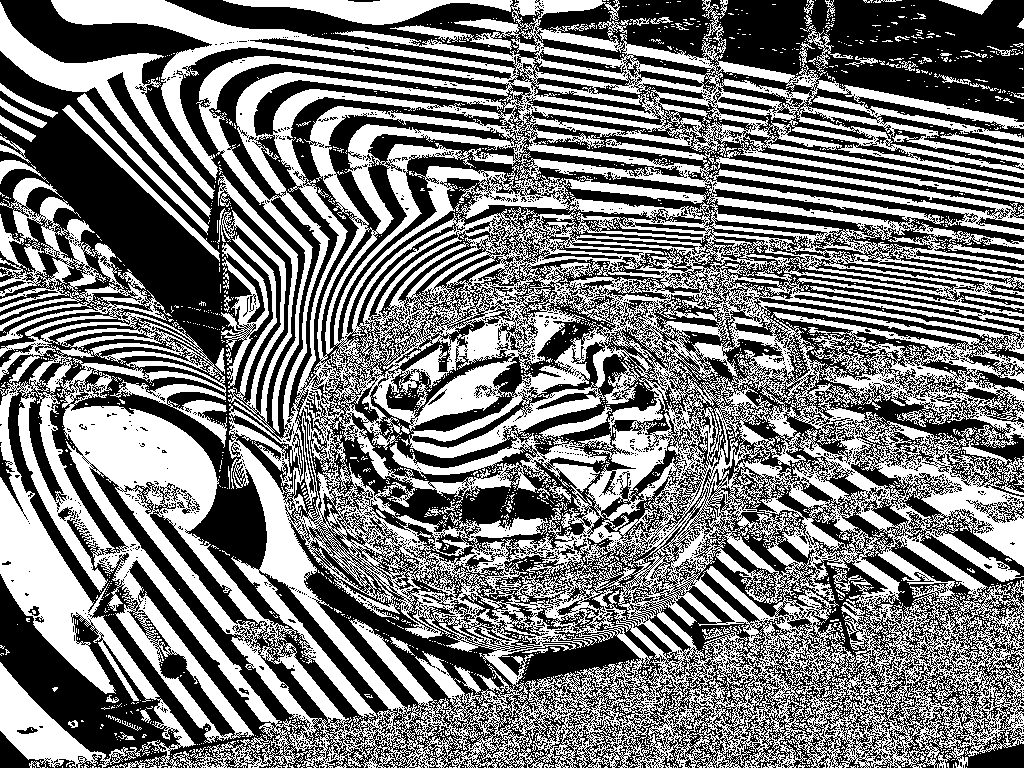
\includegraphics[width=3cm]{../out/watchm_plano0_texto1_plano_bits_1_G.png} }}%
	\qquad
	\subfloat[\centering Plano de bits 1 do canal B da Watch com mensagem escondida]{{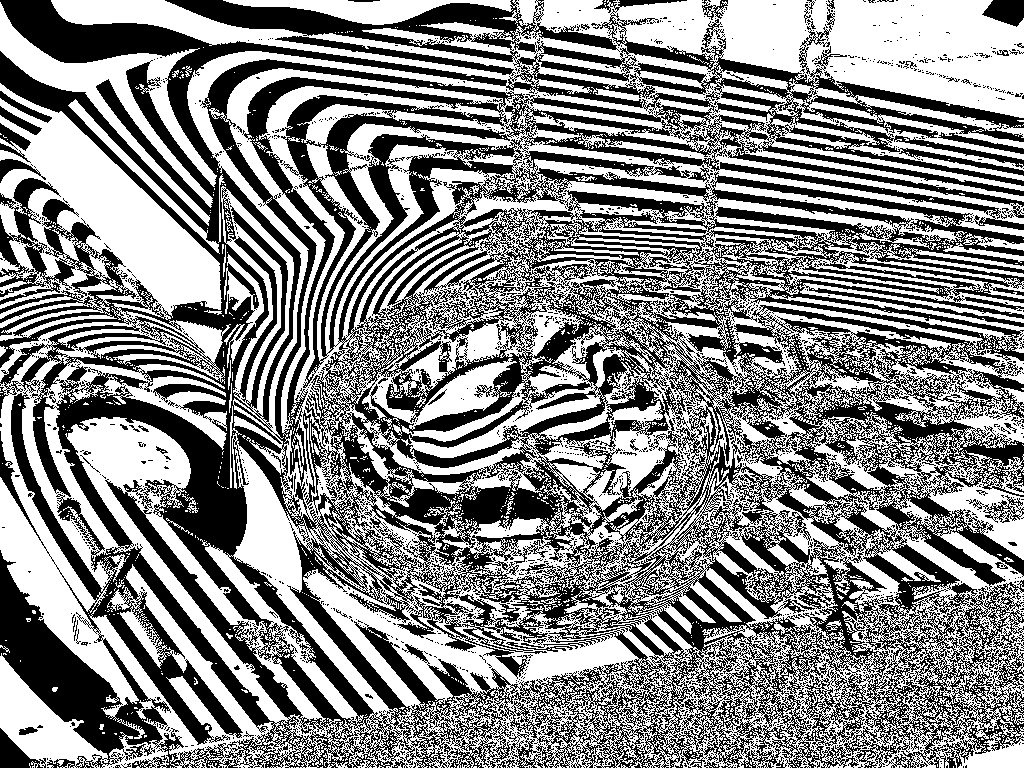
\includegraphics[width=3cm]{../out/watchm_plano0_texto1_plano_bits_1_B.png} }}%
	
	\subfloat[\centering Plano de bits 2 do canal R da Watch com mensagem escondida]{{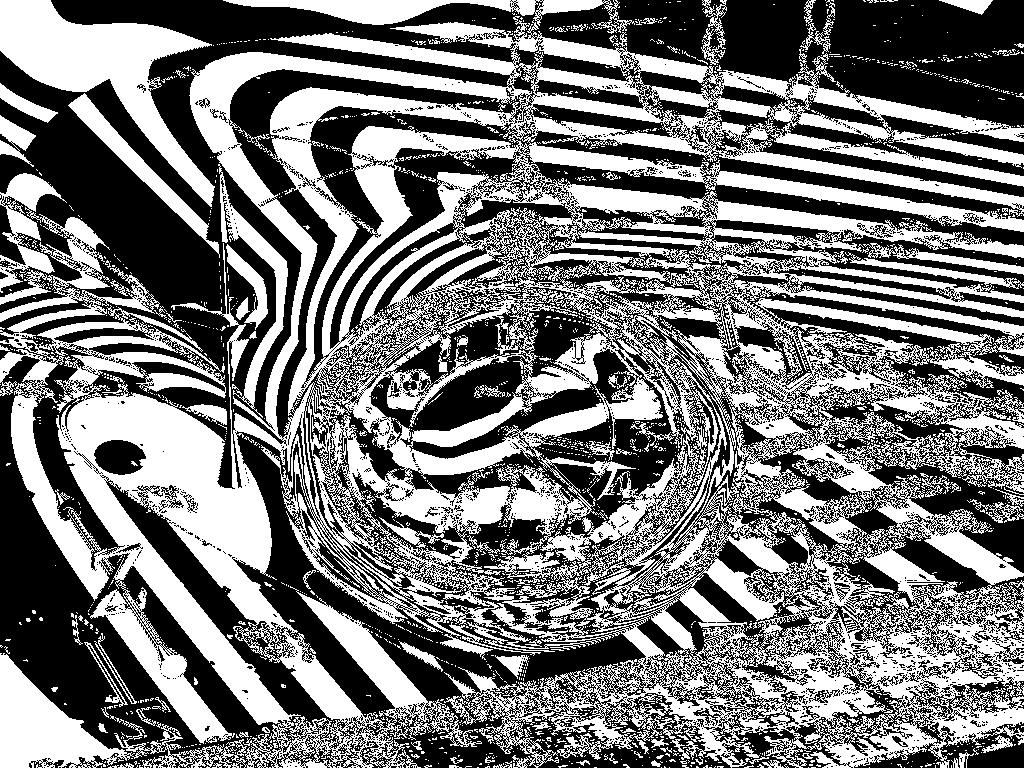
\includegraphics[width=3cm]{../out/watchm_plano0_texto1_plano_bits_2_R.png} }}%
	\qquad
	\subfloat[\centering Plano de bits 2 do canal G da Watch com mensagem escondida]{{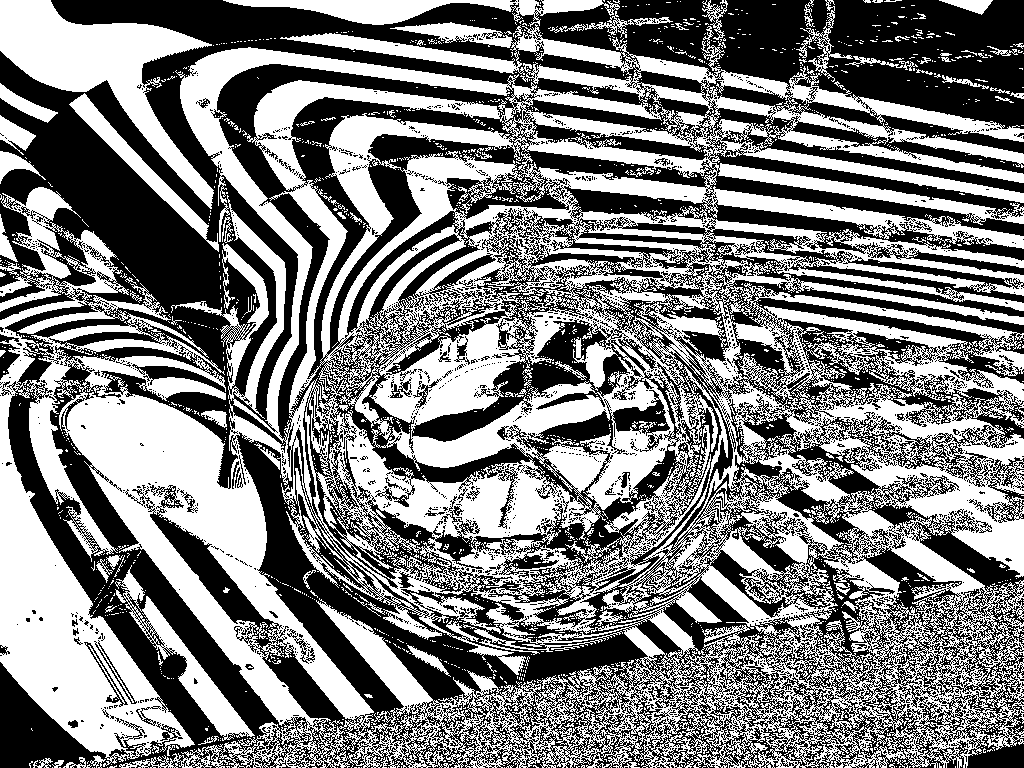
\includegraphics[width=3cm]{../out/watchm_plano0_texto1_plano_bits_2_G.png} }}%
	\qquad
	\subfloat[\centering Plano de bits 2 do canal B da Watch com mensagem escondida]{{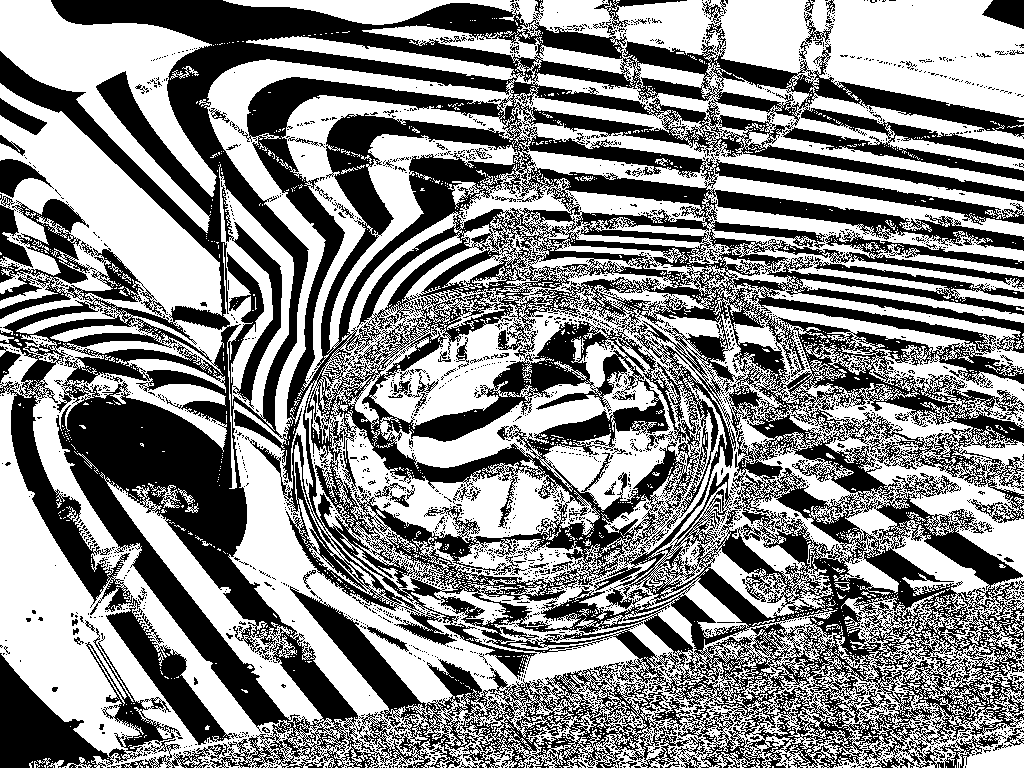
\includegraphics[width=3cm]{../out/watchm_plano0_texto1_plano_bits_2_B.png} }}%
	
	\subfloat[\centering Plano de bits 7 do canal R da Watch com mensagem escondida]{{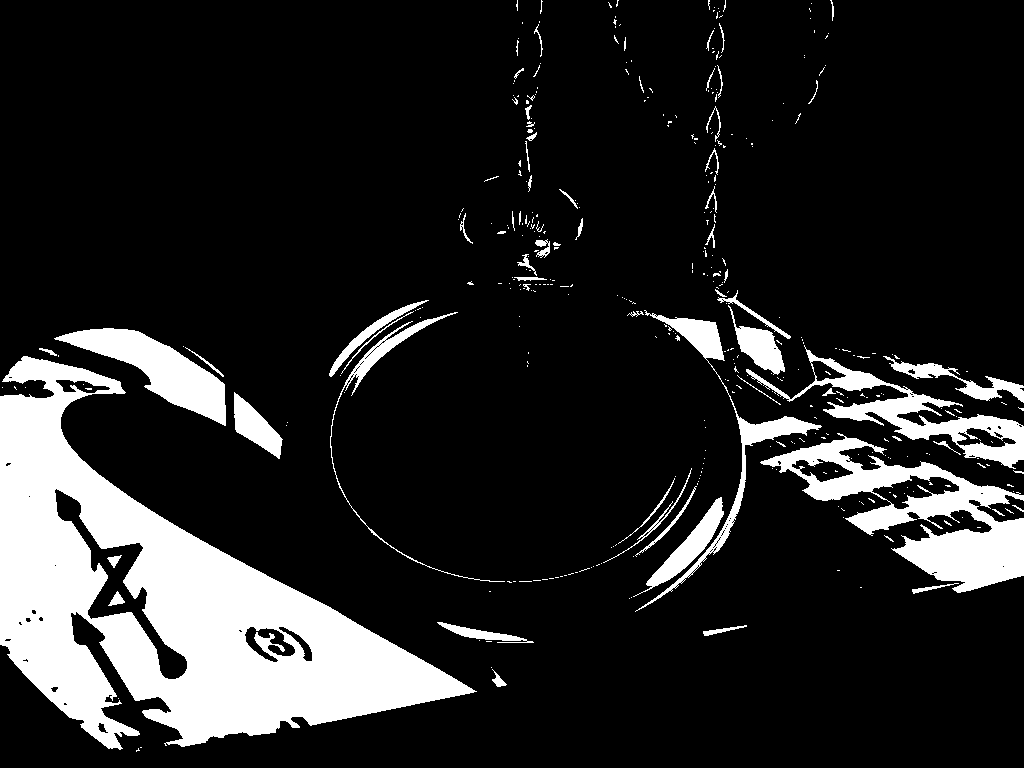
\includegraphics[width=3cm]{../out/watchm_plano0_texto1_plano_bits_7_R.png} }}%
	\qquad
	\subfloat[\centering Plano de bits 7 do canal G da Watch com mensagem escondida]{{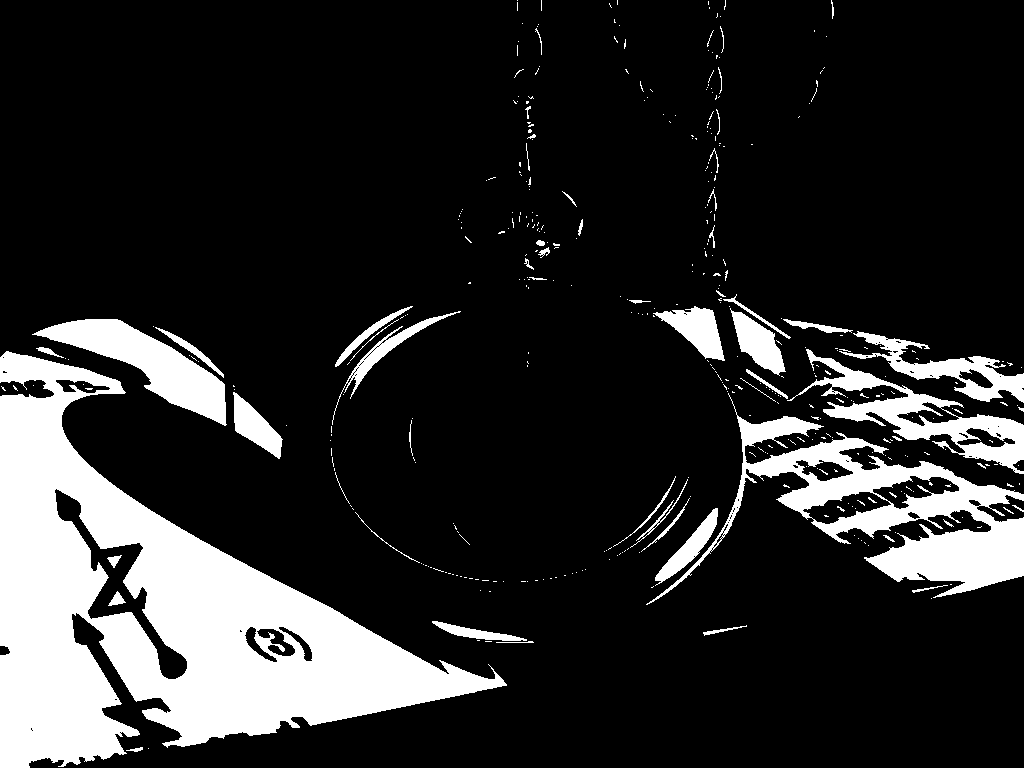
\includegraphics[width=3cm]{../out/watchm_plano0_texto1_plano_bits_7_G.png} }}%
	\qquad
	\subfloat[\centering Plano de bits 7 do canal B da Watch com mensagem escondida]{{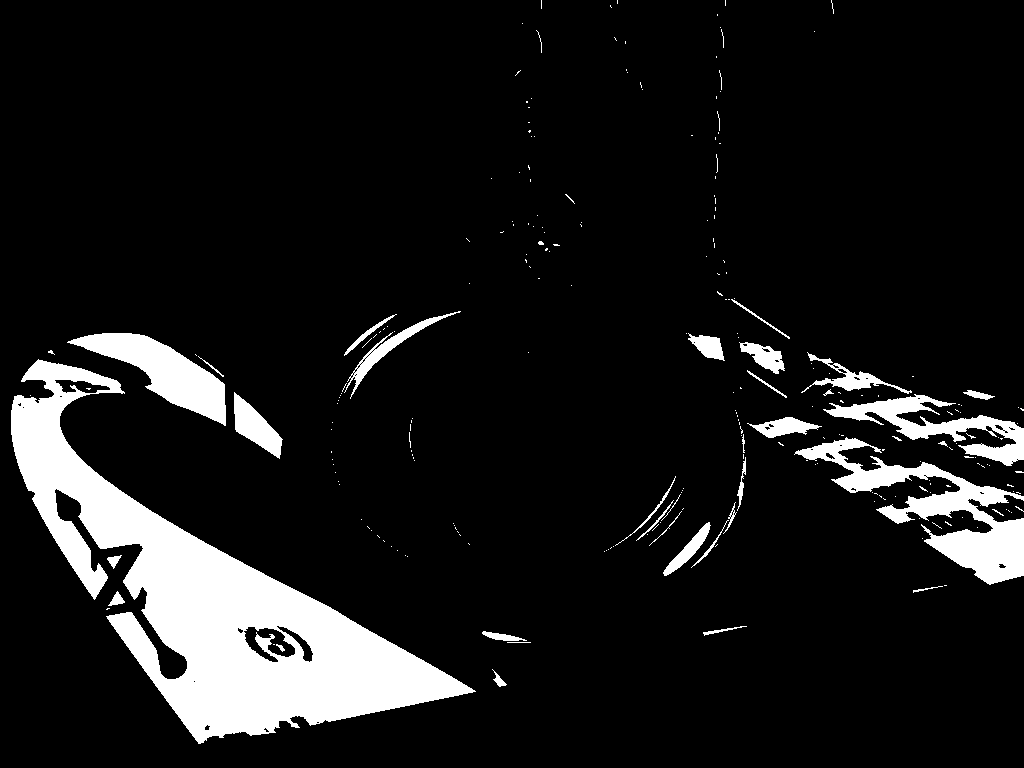
\includegraphics[width=3cm]{../out/watchm_plano0_texto1_plano_bits_7_B.png} }}%
	
	\caption{Planos de bits da imagem do Watch modificada pelos bits da mensagem do arquivo \textbf{texto1.txt}.}%
	\label{fig:imagem:plano:watch}%
\end{figure}

No caso dessa imagem, é possível notar uma alteração dos padrões de bits apresentados no seu plano de bits 0 (que é o plano onde a mensagem foi inserida). A visualização dessa quebra de padrão está dificuldade pelo tamanho da imagem, mas um olhar atento ainda é capaz de verificá-lo (olhar canto superior esquerdo da primeira linha de imagens).

\subsection{Planos de bits da imagem Baboon e Watch modifica pela mensagem contida no arquivo texto\_longo\_1.txt}

Começaremos visualizando os planos de bits da imagem do Baboon modificada. Os planos apresentados serão o 0, 1, 2, e 7 (0 menos significativo, 7 o mais significativo). As imagens dos planos de bits podem ser visualizadas na Figura \ref{fig:imagem:plano:baboon2}.

\begin{figure}[htp]%
	\centering
	\subfloat[\centering Plano de bits 0 do canal R da Baboon com mensagem escondida]{{
\includegraphics[width=3cm]{../out/baboonm_plano0_texto_longo_1_plano_bits_0_R.png} }}%
	\qquad
	\subfloat[\centering Plano de bits 0 do canal G da Baboon com mensagem escondida]{{
\includegraphics[width=3cm]{../out/baboonm_plano0_texto_longo_1_plano_bits_0_G.png} }}%
	\qquad
	\subfloat[\centering Plano de bits 0 do canal B da Baboon com mensagem escondida]{{
\includegraphics[width=3cm]{../out/baboonm_plano0_texto_longo_1_plano_bits_0_B.png} }}%
	
	\subfloat[\centering Plano de bits 1 do canal R da Baboon com mensagem escondida]{{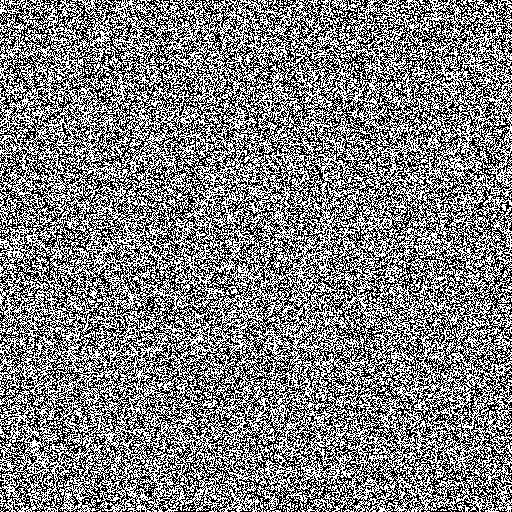
\includegraphics[width=3cm]{../out/baboonm_plano0_texto_longo_1_plano_bits_1_R.png} }}%
	\qquad
	\subfloat[\centering Plano de bits 1 do canal G da Baboon com mensagem escondida]{{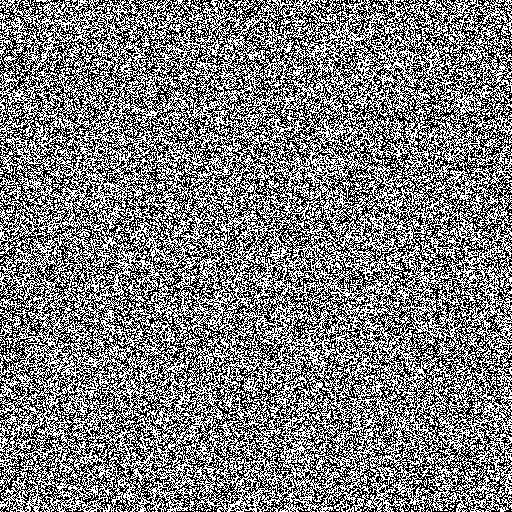
\includegraphics[width=3cm]{../out/baboonm_plano0_texto_longo_1_plano_bits_1_G.png} }}%
	\qquad
	\subfloat[\centering Plano de bits 1 do canal B da Baboon com mensagem escondida]{{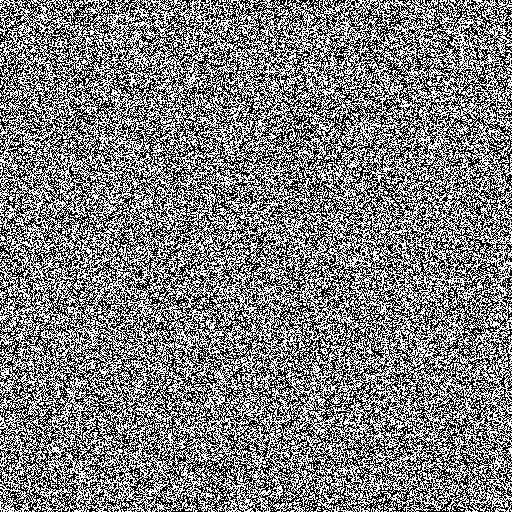
\includegraphics[width=3cm]{../out/baboonm_plano0_texto_longo_1_plano_bits_1_B.png} }}%
	
	\subfloat[\centering Plano de bits 2 do canal R da Baboon com mensagem escondida]{{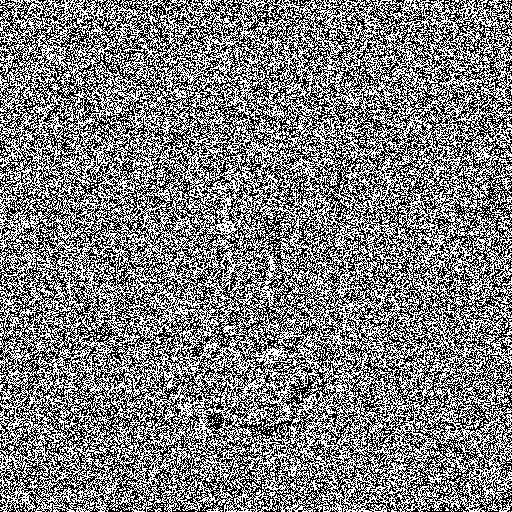
\includegraphics[width=3cm]{../out/baboonm_plano0_texto_longo_1_plano_bits_2_R.png} }}%
	\qquad
	\subfloat[\centering Plano de bits 2 do canal G da Baboon com mensagem escondida]{{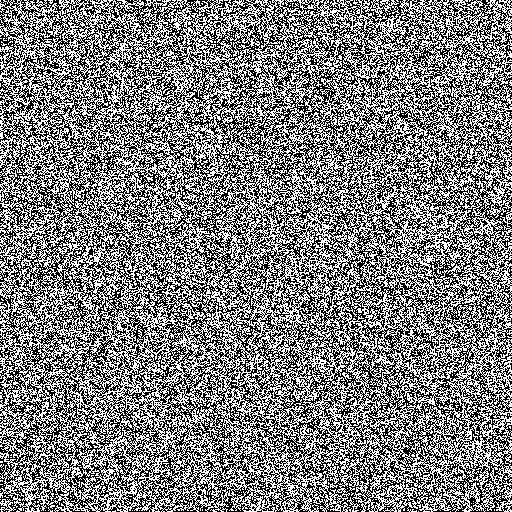
\includegraphics[width=3cm]{../out/baboonm_plano0_texto_longo_1_plano_bits_2_G.png} }}%
	\qquad
	\subfloat[\centering Plano de bits 2 do canal B da Baboon com mensagem escondida]{{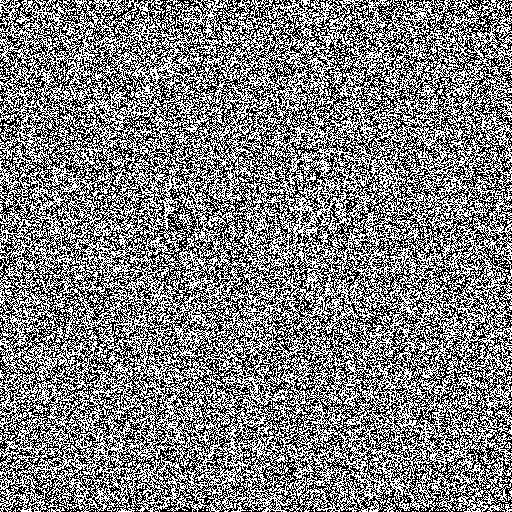
\includegraphics[width=3cm]{../out/baboonm_plano0_texto_longo_1_plano_bits_2_B.png} }}%
	
	\subfloat[\centering Plano de bits 7 do canal R da Baboon com mensagem escondida]{{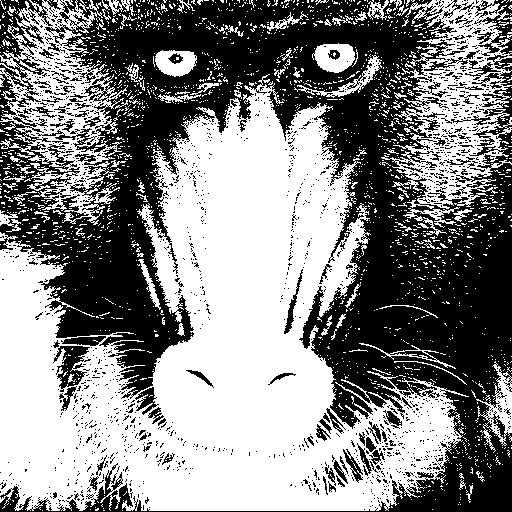
\includegraphics[width=3cm]{../out/baboonm_plano0_texto_longo_1_plano_bits_7_R.png} }}%
	\qquad
	\subfloat[\centering Plano de bits 7 do canal G da Baboon com mensagem escondida]{{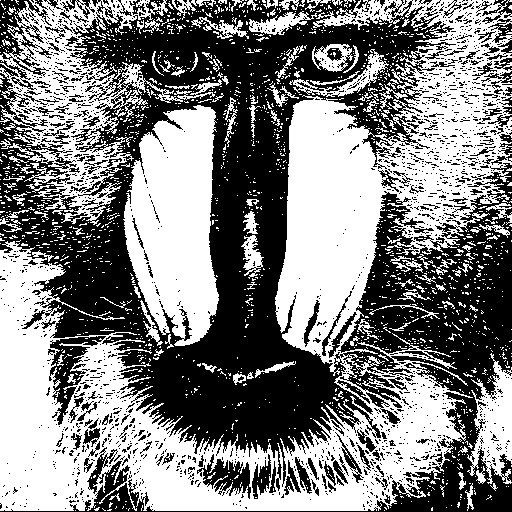
\includegraphics[width=3cm]{../out/baboonm_plano0_texto_longo_1_plano_bits_7_G.png} }}%
	\qquad
	\subfloat[\centering Plano de bits 7 do canal B da Baboon com mensagem escondida]{{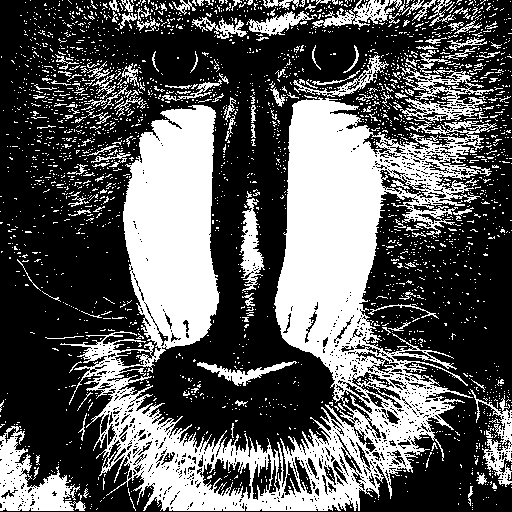
\includegraphics[width=3cm]{../out/baboonm_plano0_texto_longo_1_plano_bits_7_B.png} }}%
	
	\caption{Planos de bits da imagem do Baboon modificada pelos bits da mensagem do arquivo \textbf{texto\_longo\_1.txt}.}%
	\label{fig:imagem:plano:baboon2}%
\end{figure}

Para as imagens apresentadas na Figura \ref{fig:imagem:plano:baboon2}, notamos que é possível visualmente verificar que a imagem foi modificada a partir da análise visual dos seus planos de bits. Logo, para mensagens muito grandes, pode-se constatar que é possível verificar que uma imagem foi modificada pela análise dos padrões dos seus planos de bits.

\newpage
Agora vamos verificar o planos de bits 0, 1, 2 e 7 da imagem Watch modificada. Esses planos de bits estão apresentados na Figura \ref{fig:imagem:plano:watch2}. 

\begin{figure}[htp]%
	\centering
	\subfloat[\centering Plano de bits 0 do canal R da Watch com mensagem escondida]{{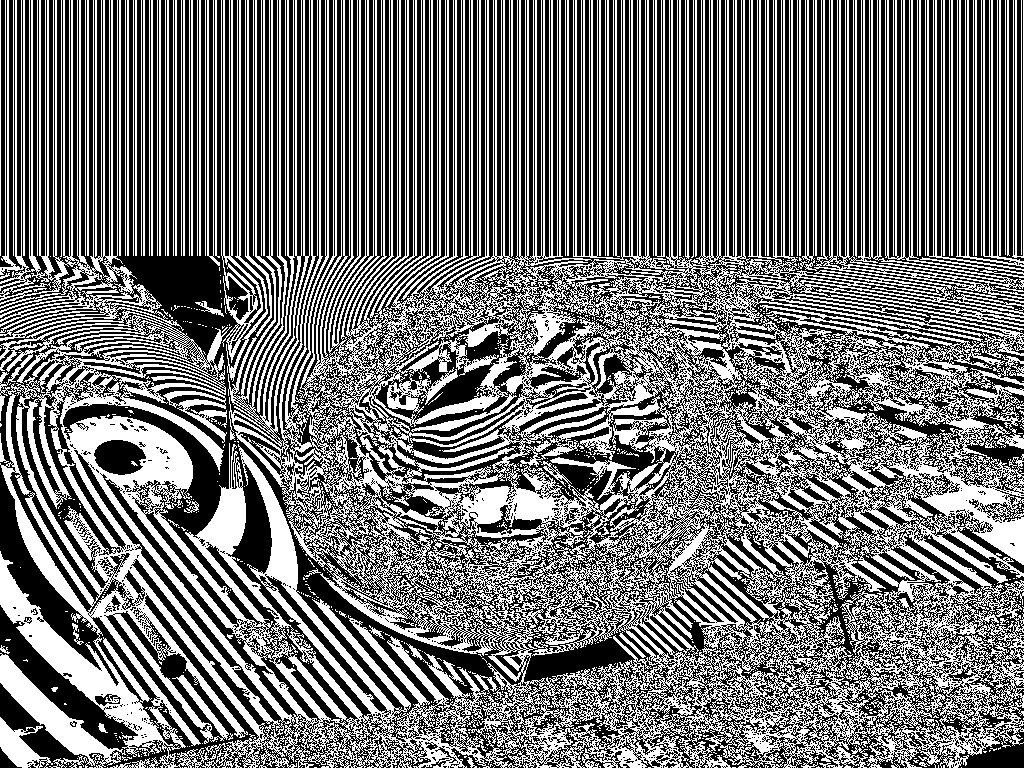
\includegraphics[width=3cm]{../out/watchm_plano0_texto_longo_1_plano_bits_0_R.png} }}%
	\qquad
	\subfloat[\centering Plano de bits 0 do canal G da Watch com mensagem escondida]{{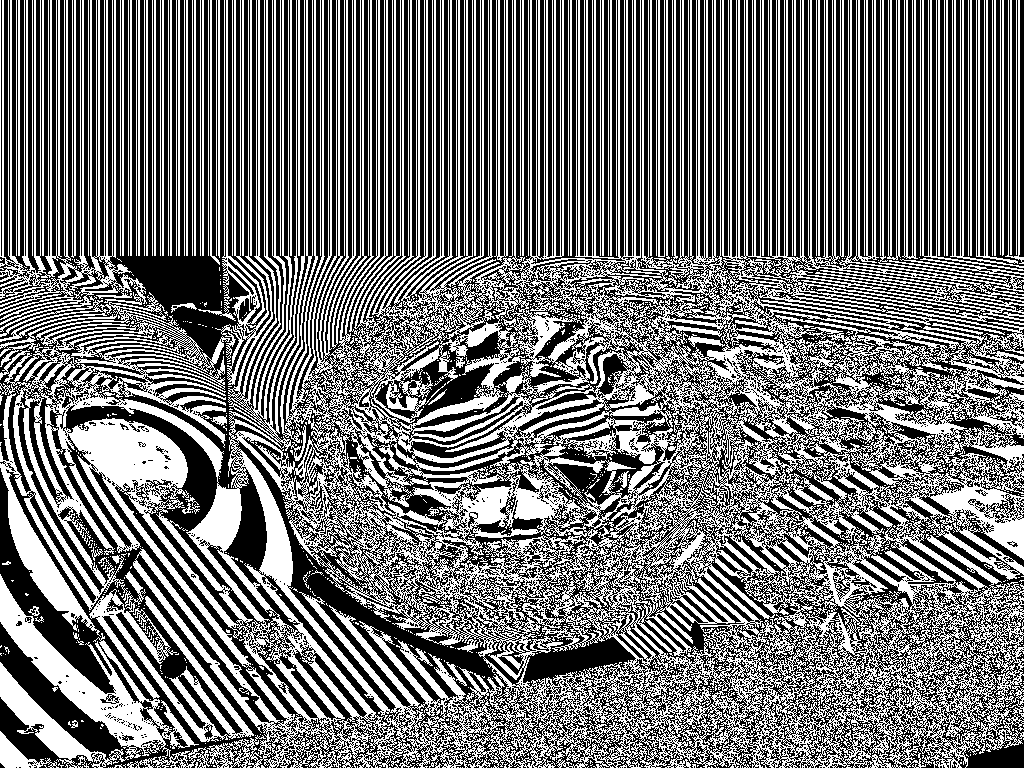
\includegraphics[width=3cm]{../out/watchm_plano0_texto_longo_1_plano_bits_0_G.png} }}%
	\qquad
	\subfloat[\centering Plano de bits 0 do canal B da Watch com mensagem escondida]{{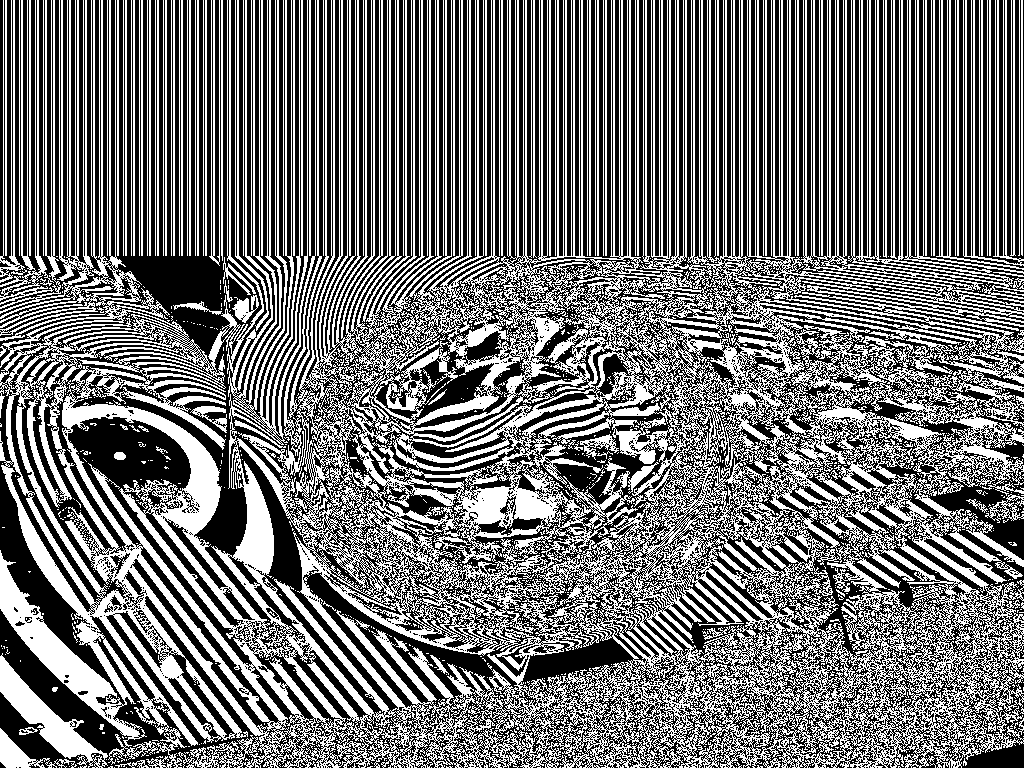
\includegraphics[width=3cm]{../out/watchm_plano0_texto_longo_1_plano_bits_0_B.png} }}%
	
	\subfloat[\centering Plano de bits 1 do canal R da Watch com mensagem escondida]{{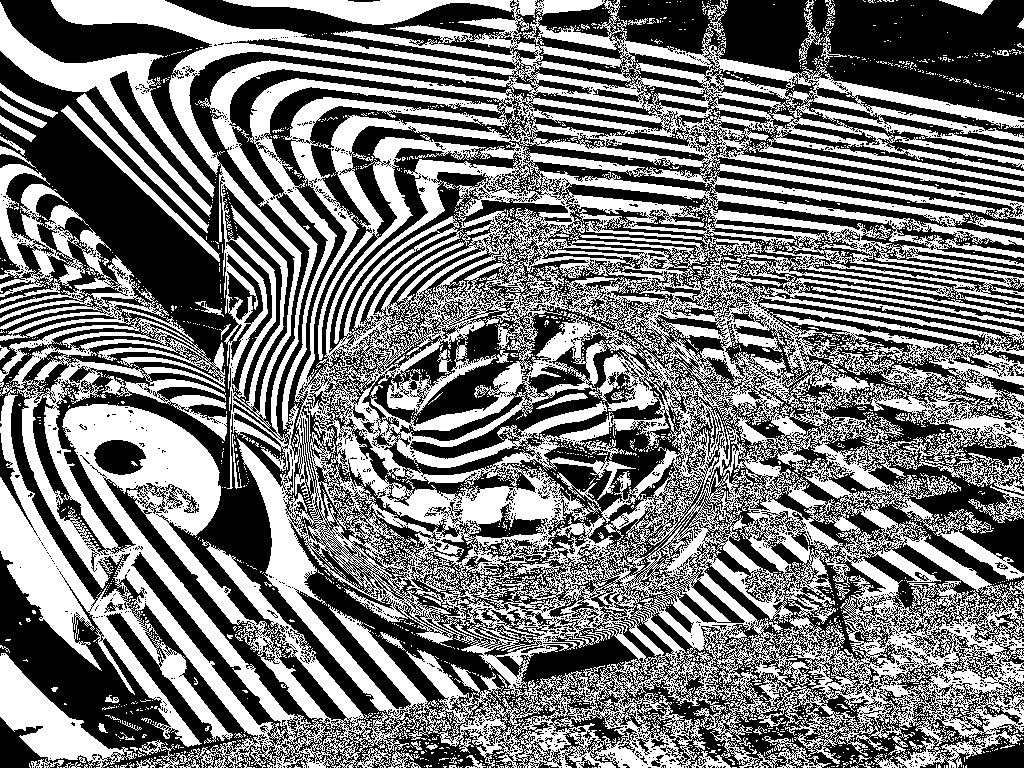
\includegraphics[width=3cm]{../out/watchm_plano0_texto_longo_1_plano_bits_1_R.png} }}%
	\qquad
	\subfloat[\centering Plano de bits 1 do canal G da Watch com mensagem escondida]{{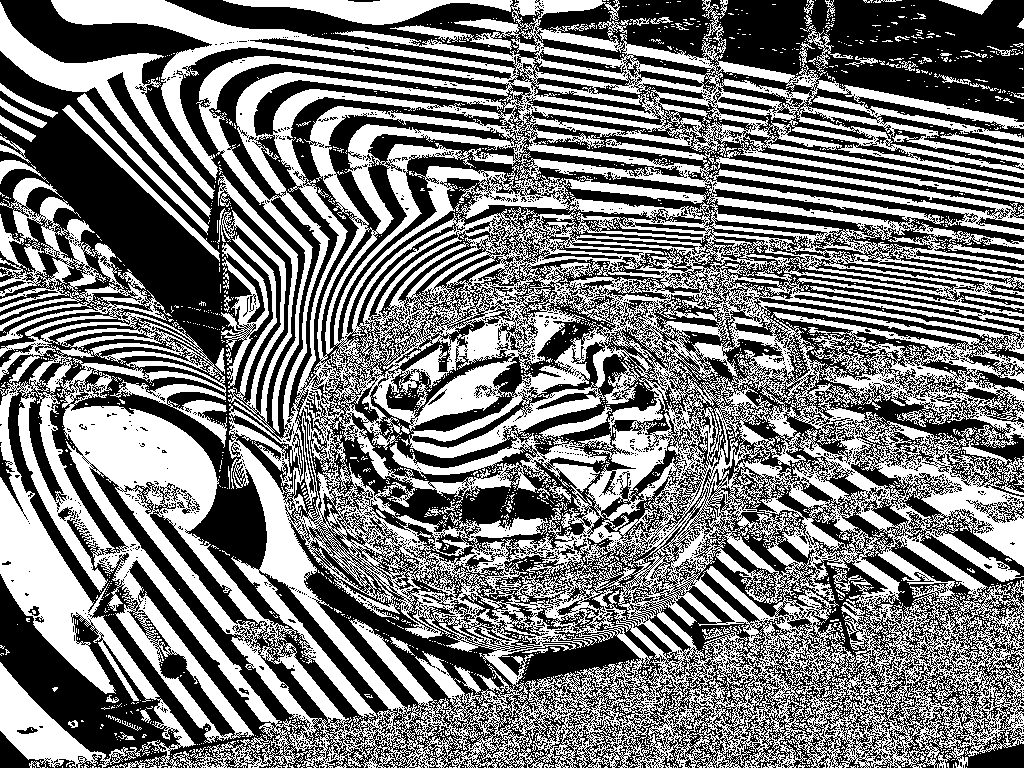
\includegraphics[width=3cm]{../out/watchm_plano0_texto_longo_1_plano_bits_1_G.png} }}%
	\qquad
	\subfloat[\centering Plano de bits 1 do canal B da Watch com mensagem escondida]{{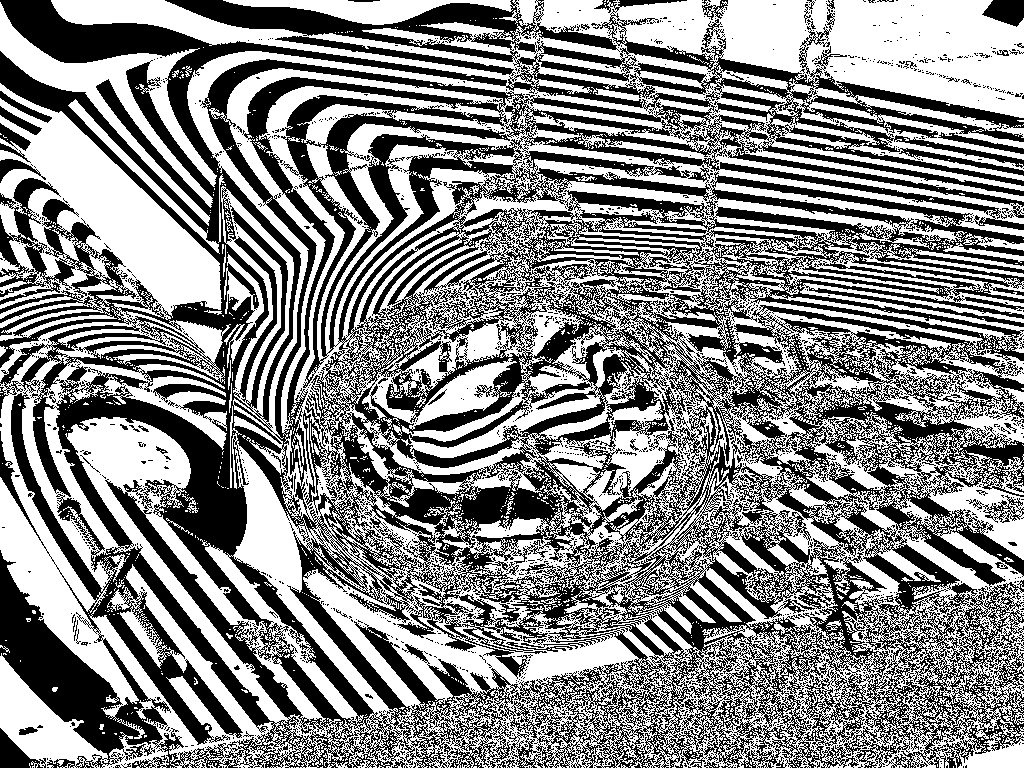
\includegraphics[width=3cm]{../out/watchm_plano0_texto_longo_1_plano_bits_1_B.png} }}%
	
	\subfloat[\centering Plano de bits 2 do canal R da Watch com mensagem escondida]{{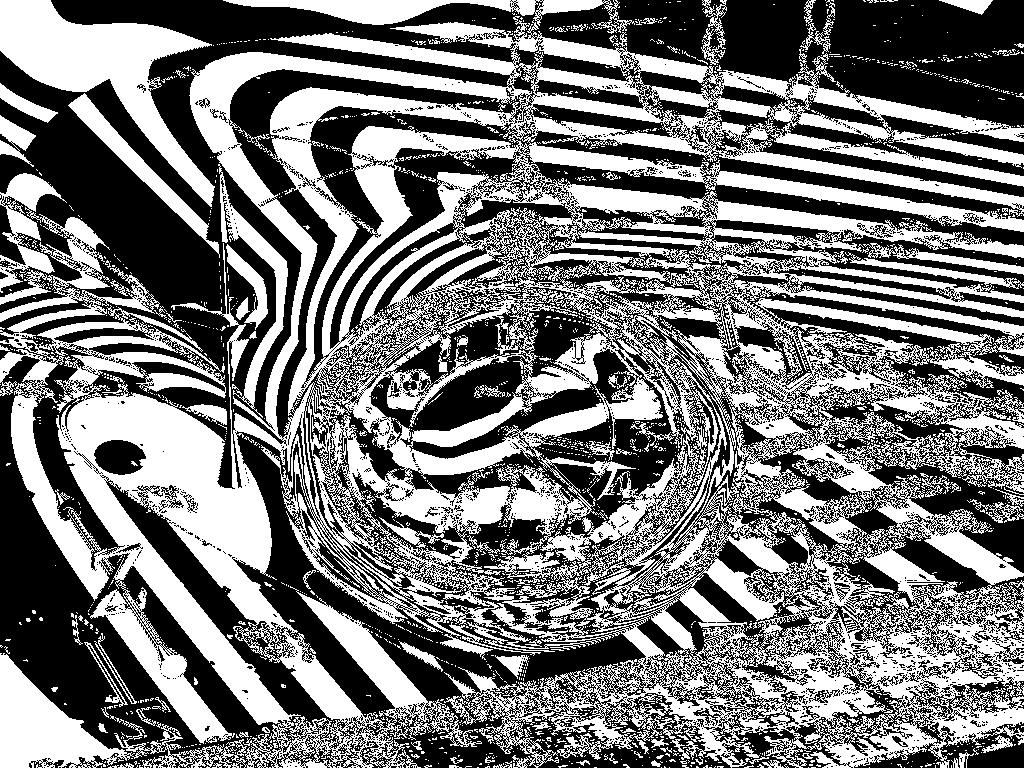
\includegraphics[width=3cm]{../out/watchm_plano0_texto_longo_1_plano_bits_2_R.png} }}%
	\qquad
	\subfloat[\centering Plano de bits 2 do canal G da Watch com mensagem escondida]{{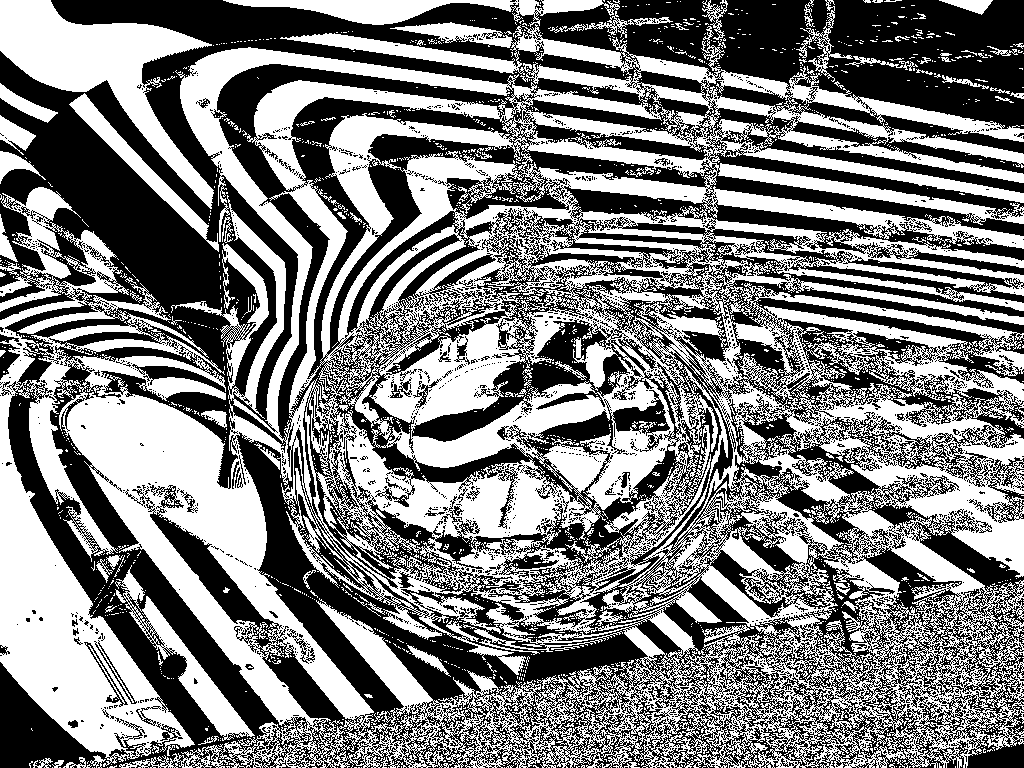
\includegraphics[width=3cm]{../out/watchm_plano0_texto_longo_1_plano_bits_2_G.png} }}%
	\qquad
	\subfloat[\centering Plano de bits 2 do canal B da Watch com mensagem escondida]{{\includegraphics[width=3cm]{../out/watchm_plano0_texto_longo_1_plano_bits_2_B.png} }}%
	
	\subfloat[\centering Plano de bits 7 do canal R da Watch com mensagem escondida]{{\includegraphics[width=3cm]{../out/watchm_plano0_texto_longo_1_plano_bits_7_R.png} }}%
	\qquad
	\subfloat[\centering Plano de bits 7 do canal G da Watch com mensagem escondida]{{\includegraphics[width=3cm]{../out/watchm_plano0_texto_longo_1_plano_bits_7_G.png} }}%
	\qquad
	\subfloat[\centering Plano de bits 7 do canal B da Watch com mensagem escondida]{{\includegraphics[width=3cm]{../out/watchm_plano0_texto_longo_1_plano_bits_7_B.png} }}%
	
	\caption{Planos de bits da imagem do Watch modificada pelos bits da mensagem do arquivo \textbf{texto\_longo\_1.txt}.}%
	\label{fig:imagem:plano:watch2}%
\end{figure}

Neste caso, assim como no anterior, é possível notar uma alteração dos padrões de bits apresentados no seu plano de bits 0 (que é o plano onde a mensagem foi inserida).

\subsection{Recuperação das mensagens}
A recuperação das mensagens escondidas pode ser feita pela execução do programa \textbf{decodificar.py}. Para as codificações realizadas anteriormente os seguintes comandos para decodificar podem ser utilizados:

\lstinline{python3 decodificar.py -imagem_entrada=out/baboonm_plano0_texto1.png -planos_bits=0};

\lstinline{python3 decodificar.py -imagem_entrada=out/watchm_plano0_texto1.png -planos_bits=0};

\lstinline{python3 decodificar.py -imagem_entrada=out/baboonm_plano0_texto_longo_1.png -planos_bits=0};

\lstinline{python3 decodificar.py -imagem_entrada=out/watchm_plano0_texto_longo_1.png -planos_bits=0}.

\noindent
As mensagens recuperadas das imagens são salvas na pasta \textbf{out} que está dentro da pasta do projeto \textbf{trab1}.

\section{Conclusão}
Do apresentado neste trabalho, podemos concluir que a esteganografia é uma técnica interessante e promissora de ocultação de mensagens em imagens sem que estas apresentem modificações visuais ao olho humano. De qualquer maneira, mesmo que visualmente as imagens não sejam alteradas, verificamos que ainda sim é possível identificar que a imagem está modifica e, assim, possivelmente com alguma mensagem escondida. Neste trabalho, essa verificação foi feita pela análise dos planos de bits das imagens modificadas. Nesse verificação, foi possível visualizar uma alteração do padrão de bits do plano de bits 0 (plano onde foi inserida a mensagem) em ambas as imagens Baboon e Watch utilizadas. A única exceção aconteceu com a imagem Baboon e a mensagem escondida \textbf{texto1.txt} que se deu, principalmente, porque a mensagem utilizada é muito pequena.


\end{document}